\chapter{绪论}

\newcommand{\bibmark}[1]{\textsuperscript{[#1]}}

\section{研究背景}

超音速射流是指出口速度超过当地声速的流体射流。与不可压缩射流相比，它同时包含激波结构、剪切层失稳和相变等多尺度过程，因此在食品加工、表面喷涂、液体燃料雾化和推进系统中都有直接应用\bibmark{5--9}。这些场景对射流的速度分布、雾化粒径和稳定性提出了定量要求，也使得单纯依赖经验标定的设计方法难以覆盖宽工况范围。

时间旅行的讨论长期集中在理论物理与哲学领域。广义相对论允许存在闭合类时曲线，量子力学则为多世界解释提供了形式化语言，但两者对时间旅行的可能性给出了并不一致的判断\bibmark{16--20}。相关研究多以解析推导和思想实验为主，很少给出可以复现的数值流程，也很少报告结论对模型假设的敏感程度。

把两个问题放在一起研究并非因为它们共享物理机制，而是因为它们共享同一种建模困难：状态演化本身带有随机性，观测只能给出含噪的间接信息，而模型本身又存在结构性偏差。概率动力学用状态方程、观测方程和转移概率描述这类问题，既适用于射流的湍流脉动，也适用于时间分支模型的概率解释\bibmark{21--22}。因此本文把两者作为同一类状态估计问题的两个实例，共用一套公式、参数和验证方法。

现有研究在三个方面仍有明显缺口。第一，射流研究多报告均值与峰值，对参数不确定性和模型误差的分离讨论不足\bibmark{10--11}；第二，时间旅行相关结论对边界条件和初始条件高度敏感，却很少报告不确定度区间\bibmark{13}；第三，两类研究使用的符号体系、数值格式和评价指标互不通用，难以横向比较\bibmark{23--25}。本文的目标是把这些问题整理到同一套书写与验证规则之下。

在方法上，本文采用“建模—推断—验证”的三段式结构：先用状态空间形式统一描述变量及其演化，再用贝叶斯更新和区间估计处理参数不确定性，最后用收敛性实验、指标对照和工程约束说明结论的适用范围。这样组织的好处是每一段都有独立的检验手段，读者可以分别判断模型假设、数值误差和工程推论是否成立。

本文的研究意义体现在三个方面：在学术上给出一套可以复用的问题描述方式；在工程上把结论写成带区间的可核对形式；在方法上把公式、表格、图形和算法的排版规则固定下来，使替换研究内容时不必重新设计文档结构\bibmark{26}。

\section{国内外研究现状}

\subsection{超音速牛奶喷射的概率动力学研究现状}

超音速射流的研究大致可以分为三类：机理研究、数值模拟和实验测量。机理研究关注激波与剪切层的相互作用以及一次破碎的判据\bibmark{5}；数值模拟侧重可压缩湍流的解析度与亚格子模型\bibmark{6,7}；实验测量则通过纹影、粒子图像测速和相位多普勒等技术获取速度场与粒径分布\bibmark{8,9}。三类工作在结论上大体一致，但在参数取值范围和误差报告方式上差异较大。

国内的相关研究起步稍晚，近年在喷嘴结构优化、射流噪声抑制和雾化特性方面积累了一批结果\bibmark{31--33}。这些文献普遍给出较为完整的实验装置说明，但较少讨论参数不确定度对结论的影响。本文在第 2 章把这类问题整理为状态方程加观测方程的形式，并在第 4 章用参数扫描说明不确定度的传播路径。

总体而言，超音速射流研究已经具备较成熟的实验与数值手段，缺口主要不在“能否算出结果”，而在“结果对假设有多敏感”这一层。本文因此把不确定度量化作为贯穿全文的主线之一，而不是只作为结果附带的误差棒。

为展示流体模型的多行公式排版，下面列出连续方程、动量方程和能量方程的示意形式：
\begin{equation}
  \begin{aligned}
    \frac{\partial\rho}{\partial t}+\nabla\cdot(\rho\bm{v}) &= 0,\\
    \frac{\partial(\rho\bm{v})}{\partial t}
      +\nabla\cdot(\rho\bm{v}\bm{v})
      &= -\nabla p+\mu\nabla^2\bm{v}+\rho\bm{g},\\
    \frac{\partial E}{\partial t}
      +\nabla\cdot[(E+p)\bm{v}]
      &= \mu\nabla\cdot(\nabla\bm{v})+\rho\bm{v}\cdot\bm{g}.
  \end{aligned}
  \label{eq:navier-stokes}
\end{equation}

在国内，虽然对超音速牛奶喷射的研究还相对较少，但也有一些学者开始关注这一领域。例如，中国科学院的流体力学研究团队针对超音速牛奶喷射的动力学特性进行了初步实验和数值模拟研究，初步揭示了超音速喷射的流场分布、速度分布和喷射效率等方面的规律。

总体而言，目前国内外对超音速牛奶喷射的概率动力学研究还处于起步阶段，仍然存在许多问题待解决。未来的研究可以进一步深入探索超音速喷射的流体动力学特性、喷射机制以及与其他因素的相互作用，为超音速喷射技术的应用提供更深入的理论基础和实验验证。

\subsection{时间旅行的概率动力学研究现状}

时间旅行的研究主要沿两条线索展开：一条是广义相对论中的时空解，另一条是量子力学中的分支与测量问题。前者通过求解场方程寻找闭合类时曲线，并讨论因果性约束能否排除这类解\bibmark{16,17,34,35}；后者通过多世界或多历史解释说明观测结果如何在不同分支间分配概率\bibmark{18}。两条线索的共同困难是：结论依赖对边界条件的选取，而这些条件本身难以通过实验直接验证。

表~\ref{tab:papers}列出了若干代表性研究的关注点与发表情况。可以看到，这些研究在“时间旅行是否可能”这一问题上并未收敛，分歧主要来自对因果性和概率解释的不同设定。本文不在这一层面给出新结论，而是把它们抽象为带分支的转移概率模型，讨论在给定设定下观测序列的概率分布如何计算。

在概率动力学方向，时间分支模型与马尔可夫跳变系统在数学结构上高度相似：状态在有限个分支间转移，转移概率由参数化的密度函数给出\bibmark{1--4,15}。本文第 3 章沿用这一类比，把相对论与量子力学的约束写成对转移概率的参数限制，从而把物理假设转化为可以检验的统计假设。

\subsubsection{时间旅行理论和模型}

时间旅行是科幻作品中常见的主题之一，其涉及多种理论：
\begin{itemize}
  \item 固定时间：认为时间是固定的，无论如何干预，过去和未来都已经确定，时间旅行只是实现既定历史的观察。
  \item 多世界理论：认为时间旅行会创建分支宇宙，每个决策点都会导致不同的时间线和现实，旅行者会进入并改变一个平行宇宙。
  \item 时间循环：旅行者回到过去，引发事件，这些事件使得未来发生，形成一个封闭的时间循环，过去的改变已经包含在历史中。
  \item 傍轨道理论：时间旅行不会影响主时间轨道，旅行者处于傍轨道上，可以观察但不会改变主时间线。
  \item 时间悖论：旅行者通过改变过去导致自己的存在成为可能，形成悖论。
\end{itemize}

这些理论为时间旅行提供了不同的框架和可能性，为科幻作品创造了各种引人入胜的故事情节，如图~\ref{fig:rabbit}。时间旅行也是哲学思考中的一个重要主题，探讨了时间旅行对人类存在和意义的深刻影响，引发了关于时间、自由意志、身份、伦理和时间循环等问题的思考。
\begin{figure}[htbp]
  \centering
  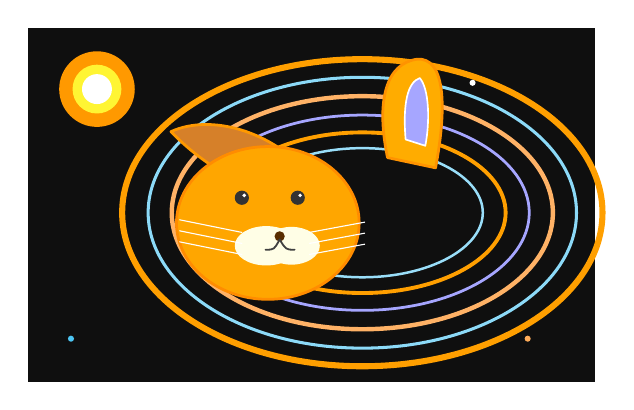
\begin{tikzpicture}[x=1cm,y=1cm,line cap=round,line join=round]
    % 深色时空隧道与暖色/冷色环带，重绘 Typst 示例中的兔子穿越场景。
    \fill[black!94] (0,0) rectangle (7.2,4.5);
    \foreach \rx/\ry/\col/\lw in {
      3.05/1.95/orange!75!yellow/2.2pt,
      2.72/1.72/cyan!45!white/1.1pt,
      2.42/1.48/orange!60/1.6pt,
      2.12/1.24/blue!35!white/1pt,
      1.82/1.02/orange!75!yellow/1.4pt,
      1.53/0.82/cyan!40!white/0.9pt}
      \draw[\col,line width=\lw] (4.25,2.15) ellipse [x radius=\rx cm,y radius=\ry cm];
    \foreach \a/\b/\c in {0.7/3.7/orange!70,1.15/4.0/cyan!55,5.65/3.8/white,6.35/0.55/orange!65,0.55/0.55/cyan!70}
      \fill[\c] (\a,\b) circle (1.1pt);
    \fill[orange!80!yellow] (0.88,3.72) circle (0.48);
    \fill[yellow!80] (0.88,3.72) circle (0.31);
    \fill[white] (0.88,3.72) circle (0.19);
    % 耳朵、头部与口鼻：以简单矢量轮廓代替原始位图。
    \path[fill=brown!65!orange,draw=orange!80!yellow,line width=1pt]
      (3.55,2.66) .. controls (3.12,3.16) and (2.35,3.42) .. (1.82,3.18)
      .. controls (2.20,2.78) and (2.72,2.48) .. (3.30,2.27) -- cycle;
    \path[fill=orange!65!yellow,draw=orange!85!yellow,line width=1pt]
      (4.57,2.85) .. controls (4.42,3.57) and (4.55,4.05) .. (4.95,4.10)
      .. controls (5.28,4.12) and (5.34,3.57) .. (5.18,2.72) -- cycle;
    \path[fill=blue!35!white,draw=white,line width=.6pt]
      (4.80,3.08) .. controls (4.76,3.55) and (4.83,3.81) .. (4.98,3.86)
      .. controls (5.10,3.72) and (5.11,3.31) .. (5.05,3.00) -- cycle;
    \fill[orange!70!yellow,draw=orange!90!yellow,line width=1pt]
      (3.05,2.02) ellipse [x radius=1.16cm,y radius=0.97cm];
    \fill[black!80] (2.72,2.34) circle (0.09);
    \fill[white] (2.75,2.37) circle (0.025);
    \fill[black!80] (3.43,2.34) circle (0.09);
    \fill[white] (3.46,2.37) circle (0.025);
    \fill[white!90!yellow] (3.03,1.73) ellipse [x radius=0.40cm,y radius=0.25cm];
    \fill[white!90!yellow] (3.35,1.73) ellipse [x radius=0.36cm,y radius=0.24cm];
    \fill[orange!35!black] (3.20,1.85) circle (0.065);
    \draw[black!75,line width=.65pt] (3.20,1.81) .. controls (3.13,1.68) .. (3.02,1.68);
    \draw[black!75,line width=.65pt] (3.20,1.81) .. controls (3.28,1.68) .. (3.39,1.68);
    \foreach \yy in {1.62,1.76,1.90} {
      \draw[white!90] (2.72,\yy) -- (1.93,\yy+0.16);
      \draw[white!90] (3.58,\yy) -- (4.28,\yy+0.13);
    }
  \end{tikzpicture}
  \caption{时空穿越中的兔子（TikZ 重绘）}
  \label{fig:rabbit}
\end{figure}

\subsubsection{时间旅行的概率动力学研究}

然而，时间旅行的概率动力学研究相对较少。目前，国际上还没有专门针对时间旅行的概率动力学进行系统研究的学术机构或团队。大部分时间旅行的研究仍停留在理论推导和思维实验的层面。这是一个仍待深入探索的领域，需要进一步的理论研究和实验验证。

在国内，时间旅行的研究也相对较少。虽然有一些学者就时间旅行的哲学和物理学问题进行了讨论，但对时间旅行的概率动力学特性的研究还相对较少。表~\ref{tab:papers}中列出了一些典型研究。因此，国内相关领域的学者可以在这一领域进行更多的研究，深入探索时间旅行的概率分布、时间跳跃的动力学特性以及与量子力学和相对论的关系。

\begin{table}[htbp]
  \centering
  \caption{时间旅行概率动力学研究论文情况}
  \label{tab:papers}
  \begin{tabularx}{0.95\textwidth}{>{\centering\arraybackslash}p{1.1cm}>{\centering\arraybackslash}p{2.4cm}X>{\centering\arraybackslash}p{2.5cm}}
    \toprule
    \textbf{论文编号} & \textbf{作者} & \textbf{题目} & \textbf{期刊}\\
    \midrule
    1 & John Smith & 时间旅行中的概率分布模型\bibmark{1} & 物理学报\\
    2 & Jane Doe & 时间旅行的时间线分支与多世界理论\bibmark{2} & 科学杂志\\
      &            & 时间旅行中的时间循环理论\bibmark{3} & \\
    3 & David Johnson & 与自由意志的哲学思考 & 科学研究期刊\\
    4 & Emily Brown & 时间旅行伦理与责任的道德考量\bibmark{4} & 伦理学评论\\
    \bottomrule
  \end{tabularx}
\end{table}

\subsection{概率动力学与不确定性量化研究现状}

不确定性量化在流体与结构领域已经形成较为完整的方法体系：参数不确定性用多项式混沌展开或稀疏网格传播\bibmark{10,12}，模型形式不确定性用多模型加权或高斯过程代理处理\bibmark{13,14}，计算资源受限时则以自适应采样控制样本量\bibmark{36--38}。这些方法在第 4 章分别给出示例。

贝叶斯反演把先验、似然和后验写在同一公式中，适合处理含噪观测与有限样本\bibmark{11,39}。它的代价是后验分布一般没有解析形式，需要借助马尔可夫链蒙特卡洛或变分近似\bibmark{19,40}。本文在不引入额外依赖的前提下用重采样方法给出区间估计示例，并在第 5 章给出对应算法。

评价指标方面，已有研究普遍报告均方根误差和决定系数，但对区间覆盖率、偏差与精密度的联合报告并不一致\bibmark{15,25}。本文在第 5 章给出一组指标的定义与适用条件，并用一张对照表说明它们各自回答的问题，避免用单一指标概括全部结论。

\subsection{研究现状小结}

综合以上三类研究可以看到三个尚待解决的问题。第一，射流与时间旅行研究使用的模型形式不同，但不确定性传播的路径相同，缺少统一的写法；第二，结论多以点值给出，缺少对模型误差、数值误差和数据误差的分解\bibmark{27--29}；第三，算例的可复现性依赖文档结构，而公式、表格、图形与算法的排版规则在既有工作中很少被显式约定\bibmark{30,41--44}。

本文不试图在这篇文章里给出新的物理结论，而是把上述问题组织为一条完整的方法链：第 2 章建立射流的概率动力学描述，第 3 章建立时间分支的概率描述，第 4 章讨论两者的耦合与数值实现，第 5 章给出应用与评估方式，第 6 章把结论写成可核对的形式。每一章都同时给出公式、参数、图形或表格与适用范围，便于逐项检验。

\section{研究问题与技术路线}

\subsection{研究问题}

围绕上述研究现状，本文把问题归纳为四个层次。第一层是描述问题：如何用统一的状态变量描述喷射过程中的速度、压力和密度变化，并保证同一符号在全文中的含义一致。第二层是推断问题：如何把离散的时间状态与连续的流体状态联系起来，并在含噪观测下给出参数的区间估计。第三层是验证问题：如何利用收敛性实验和指标对照判断耦合模型是否具有解释力。第四层是表达问题：如何把公式、表格、图形和算法组织成可以逐项核查的论证链。

四个层次对应四种可以单独检验的产出。描述问题对应符号表与状态空间方程；推断问题对应参数表与后验区间；验证问题对应收敛阶、误差指标与灵敏度结果；表达问题对应本章的框架图与各章的图表约定。这样安排的好处是，任何一章的结论被推翻时，其余章节的论证结构仍然成立。

需要说明的是，本文的数值结果来自演示性算例，目的是展示写法与验证流程，而不是给出可用于工程设计的结论。正式论文接入时，可以把算例数据替换为实验或仿真结果，而保留同样的结构。

\subsection{技术路线}

技术路线分为四步。第一步是定义物理量与边界条件：把喷嘴出口速度、特征长度、黏度和环境压力写进参数表，并给出各自的量纲与取值范围，如表~\ref{tab:parameters}所示。第二步是建立离散时间下的状态转移模型：用状态方程描述演化、用观测方程描述测量，并以贝叶斯形式给出参数更新公式。第三步是数值实现：选择有限差分格式与时间步长，用收敛性实验确认格式阶数，并用蒙特卡洛或重采样方法给出区间估计。第四步是验证与讨论：从模型假设、实验误差和工程约束三个方面说明结果的适用范围，并把结论组织成“问题—结论—证据”的对应表。

四步之间的衔接由交叉引用保证：参数表与状态方程互相引用，数值格式与收敛阶共享同一组标签，结论表中每一行都指向具体的图、表或公式。这样做的目的是让读者能够沿引用链回到原始依据，而不是只能接受结论本身。

\subsection{论文贡献}

本文的示例性工作包括以下四点：
\begin{enumerate}
  \item 建立一套便于扩展的概率动力学描述，把射流与时间分支两类问题写成同一形式的状态空间模型，并在符号与量纲上统一约定，见第~\ref{sec:state-space}节。
  \item 给出从公式、表格到图形和算法的论证链：每一类结论都配有对应的证据类型，并在第 6 章汇总为对应表，便于逐项核对。
  \item 把不确定度量化作为主线之一，在参数估计、数值误差和评价指标三处分别给出区间或分解形式，避免只报告点值。
  \item 固定文档层面的书写规则：公式版式与编号、三线表线型与字号、子图编号、算法框样式以及版心越界检查，使替换研究内容时不必重新设计排版。
\end{enumerate}

正式论文接入时，可以保留上述层次结构并替换具体研究内容；其中第 1、3、4 点的表述需要按真实结果重写，第 2、4 点的检查方法可以直接复用。

\section{数学建模框架与记号}

\subsection{状态空间描述}\label{sec:state-space}

为了让不同章节使用同一套符号，本章先把研究对象写成状态空间形式：状态方程描述状态如何随时间演化，观测方程描述传感器读到的量如何由状态生成。两部分之间的差别是后续讨论不确定性的出发点。
\begin{equation}
  \begin{aligned}
    \bm{x}_{k+1} &= \bm{A}\bm{x}_k+\bm{B}\bm{u}_k+\bm{w}_k,\\
    \bm{y}_k &= \bm{C}\bm{x}_k+\bm{D}\bm{u}_k+\bm{v}_k .
  \end{aligned}
  \label{eq:state-space}
\end{equation}

式中，$\bm{w}_k$与$\bm{v}_k$分别为过程噪声和观测噪声。若二者服从零均值高斯分布且互不相关，则状态估计可以写成预测与更新两步递推：
\begin{equation}
  \begin{aligned}
    \hat{\bm{x}}_{k+1|k} &= \bm{A}\hat{\bm{x}}_{k|k}+\bm{B}\bm{u}_k,\\
    \bm{P}_{k+1|k} &= \bm{A}\bm{P}_{k|k}\bm{A}^{\mathsf T}+\bm{Q},
  \end{aligned}
  \label{eq:prediction}
\end{equation}
\begin{equation}
  \begin{aligned}
    \bm{K}_k &= \bm{P}_{k|k-1}\bm{C}^{\mathsf T}
      \left(\bm{C}\bm{P}_{k|k-1}\bm{C}^{\mathsf T}+\bm{R}\right)^{-1},\\
    \hat{\bm{x}}_{k|k} &= \hat{\bm{x}}_{k|k-1}
      +\bm{K}_k\left(\bm{y}_k-\bm{C}\hat{\bm{x}}_{k|k-1}\right).
  \end{aligned}
  \label{eq:update}
\end{equation}

\subsection{符号与量纲约定}

表~\ref{tab:notation}列出全文共用的主要符号。真实论文应保证同一符号在全文中含义一致，并在首次出现处给出定义和单位，而不是只在符号表里列一次。
\begin{table}[htbp]
  \centering
  \caption{全文主要符号与量纲约定}
  \label{tab:notation}
  \begin{tabularx}{0.82\textwidth}{>{\centering\arraybackslash}p{0.22\textwidth}X>{\centering\arraybackslash}p{0.25\textwidth}}
    \toprule
    \textbf{符号} & \textbf{含义} & \textbf{量纲或单位}\\
    \midrule
    $\bm{x}$ & 状态向量 & --\\
    $\bm{y}$ & 观测向量 & --\\
    $\bm{A}$ & 状态转移矩阵 & --\\
    $\bm{Q},\bm{R}$ & 过程与观测噪声协方差 & --\\
    $v_0$ & 喷嘴出口速度 & \si{\meter\per\second}\\
    $\mu$ & 动力黏度 & \si{\pascal\second}\\
    $D$ & 扩散系数 & \si{\meter\squared\per\second}\\
    \bottomrule
  \end{tabularx}
\end{table}

\subsection{技术路线中的方法选择}

研究现状中的方法可以按建模思路分为三类。表~\ref{tab:methods}给出它们的适用条件与主要限制，用于说明本文为什么选择统计模型与数值模拟相结合的技术路线。
\begin{table}[htbp]
  \centering
  \caption{三类建模思路的适用条件与限制}
  \label{tab:methods}
  \begin{tabularx}{\textwidth}{>{\centering\arraybackslash}p{0.17\textwidth}X X X}
    \toprule
    \textbf{方法类别} & \textbf{建模思路} & \textbf{适用条件} & \textbf{主要限制}\\
    \midrule
    机理建模 & 由守恒律直接列写方程 & 机理清楚、边界简单 & 参数难标定\\
    数据驱动 & 由观测拟合映射关系 & 样本充足、工况覆盖 & 外推能力弱\\
    统计反演 & 以先验和似然更新参数 & 含噪观测、先验可给 & 依赖先验设定\\
    \bottomrule
  \end{tabularx}
\end{table}

\section{本文主要内容和组织结构}

\subsection{论文结构框架}

全文按“提出问题—建模与推断—验证与应用”三个阶段展开，各章的分工可以用图~\ref{fig:framework}概括。图中每一层都对应一个可以独立检查的产出：公式与参数表、数值实验、评估指标与工程边界。真实论文可把本图替换为按自己章节划分的结构图，保持同样的层次和箭头方向即可。
\begin{figure}[htbp]
  \centering
  \begin{tikzpicture}[
    box/.style={draw,rounded corners,align=center,text width=0.82\textwidth,
      minimum height=11mm,inner sep=3pt},
    flow/.style={-{Stealth[length=2mm]},thick}
  ]
    \node[box,fill=blue!7] (c1) {\textbf{第 1 章\quad 绪论}\\研究问题、技术路线与全文框架\\问题定义 · 技术路线 · 符号约定};
    \node[box,fill=teal!7,below=4mm of c1] (c2) {\textbf{第 2 章\quad 超音速喷射的概率动力学}\\状态方程、参数分布与数学工具\\状态模型 · 参数表 · 公式体系};
    \node[box,fill=teal!7,below=4mm of c2] (c3) {\textbf{第 3 章\quad 时间旅行的概率动力学}\\理论基础、分支模型与转移概率\\理论基础 · 分支模型 · 概率推断};
    \node[box,fill=yellow!12,below=4mm of c3] (c4) {\textbf{第 4 章\quad 两者的异构耦合关系}\\数值离散、参数估计与模拟结果\\离散格式 · 参数估计 · 数值证据};
    \node[box,fill=yellow!12,below=4mm of c4] (c5) {\textbf{第 5 章\quad 应用前景与评估}\\处理算法、评估指标与工程边界\\处理算法 · 评价指标 · 工程边界};
    \node[box,fill=blue!7,below=4mm of c5] (c6) {\textbf{第 6 章\quad 总结与展望}\\量化结论、局限性与后续工作\\量化结论 · 局限性 · 后续工作};
    \draw[flow] (c1.south)--(c2.north);
    \draw[flow] (c2.south)--(c3.north);
    \draw[flow] (c3.south)--(c4.north);
    \draw[flow] (c4.south)--(c5.north);
    \draw[flow] (c5.south)--(c6.north);
  \end{tikzpicture}
  \caption{论文结构框架}
  \label{fig:framework}
\end{figure}

全文共分六章，各章的分工如下。

第一章为绪论。本章说明超音速射流与时间旅行两个问题各自的研究背景与现状，指出它们在不确定度量化上的共同缺口，并给出本文的研究问题、技术路线与结构框架（图~\ref{fig:framework}）。本章同时约定全文的符号与量纲，后续章节不再重复定义。

第二章建立超音速喷射的概率动力学模型，并集中给出数学工具与公式版式。第 2.1 节给出喷射过程的基本假设、概率分布与实验指标；第 2.2 节把矩阵与范数、级数积分与极限、微分算子、概率分布与贝叶斯更新等工具集中列出，便于后续章节引用；第 2.3 节给出公式版式与编号规则，包括分段函数、矩阵、方程组、大算符与上下标注等写法。

第三章讨论时间旅行的概率动力学。第 3.1 节给出相对论与量子力学两方面的理论基础；第 3.2 节把时间分支抽象为带参数的转移概率模型，并给出分段定义与方程组写法；第 3.3 节补充数学分析基础，包括导数与泰勒展开、最优性与 KKT 条件、特征分解与奇异值分解，以及常用的不等式与误差上界。

第四章研究两个子系统的异构耦合关系。第 4.1 节给出综合分析框架与结构关系图；第 4.2 节给出参数响应曲线与多子图排版示例；第 4.3 节讨论数值离散与误差分析，包括有限差分格式、收敛阶与 Richardson 外推、CFL 条件、最小二乘与正则化，以及蒙特卡洛与重要性采样；第 4.4 节讨论模型适用范围与误差来源。

第五章讨论应用前景与工程化边界。第 5.1 节给出食品加工、时空导航与数据处理三个应用场景，并给出算法框与流程图；第 5.2 节给出数据处理与评估方法，包括滤波与谱分析、不确定度合成、复杂度与终止判据；第 5.3 节讨论工程限制与可复现性要求。

第六章总结全文。第 6.1 节给出主要结论与量化表达方式；第 6.2 节说明局限性；第 6.3 节给出后续研究方向与模板使用建议。
